\documentclass{article}
%packages
\usepackage{graphicx}
\usepackage[utf8]{inputenc}
\usepackage[T1]{fontenc}
\usepackage[frenchb]{babel}
\usepackage[a4paper]{geometry}
\usepackage{minted}

\newcommand{\bitem}{\item[\textbullet]}

\begin{document}
%title
\begin{titlepage}
	\vspace{-20px}
	\begin{tabular}{l}
		\textsc{Blin} S\'ebastien\\
		\textsc{Collin} Pierre-Henri
	\end{tabular}
	\hfill \vspace{10px}
\includegraphics[scale=0.1]{esir.png}\\
	\vfill
	\begin{center}
		\Huge{\'Ecole sup\'erieure d'ing\'enieurs de Rennes}\\
		\vspace{1cm}
		\LARGE{1\`ere Ann\'ee}\\
		\large{Parcours Informatique}\\
		\vspace{0.5cm}\hrule\vspace{0.5cm}
		\LARGE{\textbf{Algorithmie des graphes}}\\
		\Large{Dossier de Spécifications - Allocateur}
		\vspace{0.5cm}\hrule
		\vfill
		\vfill
	\end{center}
	\begin{flushleft}
		\Large{Sous l'encadrement de~:}\\
		\vspace{0.2cm}
		\large{{Bateux} Quentin}
	\end{flushleft}
	\vfill
\end{titlepage}

\section{Règles et définitions supplémentaires}
\begin{itemize}
  \bitem \textbf{R12} : En cas d'interblocage, le processus ayant créé la demande menant à cet interblocage est détruit.
  \bitem \textbf{R13} : Un processus actif peut demander de nouvelles ressources même si ça mène à un interblocage.
\end{itemize}

\section{Règles de modélisation}

\subsection{Invariants}
\begin{itemize}
  \bitem \textbf{MI1} : Les sommets des graphes représentent des processus et des ressources.
  \bitem \textbf{MI2} : Les sommets de sorties du graphe représentent les ressources.
  \bitem \textbf{MI3} : Les sommets d'entrées du graphe représentent les processus actifs.
  \bitem \textbf{MI4} : Tout sommet qui n'est ni d'entrée, ni de sortie est un processus bloqué.
  \bitem \textbf{MI5} : Une demande de ressource est représenté par un arc orienté entre un sommet-processus vers un sommet-ressource.
  \bitem \textbf{MI6} : Une attente entre processus est représenté par un arc orienté du sommet-processus s'éxécutant le premier vers un sommet-processus qui s'éxécutera plus tard.
  \bitem \textbf{MI7} : Une file d'attente d'une ressource est représenté par le chemin le plus long entre le sommet-processus actif de la ressource et celle-ci.
  \bitem \textbf{MI8} : Un interblocage est modélisé par un cycle dans le graphe.
  \bitem \textbf{MI9} : L'affichage décrit par (O5) est donné par la file d'attente de la ressource (sans les processus actifs).
  \bitem \textbf{MI10} : L'affichage des attentes d'un processus est donné par les parents de celui-ci.
\end{itemize}

\subsection{Variants}
\begin{itemize}
  \bitem \textbf{MV1} : La création d'un processus entraine la création d'un sommet-processus.
  \bitem \textbf{MV2} : La destruction d'un processus actif entraîne la destruction de tous ces arcs.
  \bitem \textbf{MV3} : Si une demande provoque un interblocage, on détruit le sommet-processus venant de réaliser la demande.
  \bitem \textbf{MV4} : La demande d'une ressource libre par un processus entraine la création  d'un arc entre le sommet-processus et le sommet-ressource.
  \bitem \textbf{MV5} : La demande d'une ressource non-libre par un processus entraine la création  d'un arc entre le sommet-processus et le sommet-ressource ainsi qu'un arc orienté du dernier sommet-processus en attente par ressource demandée vers le sommet.
  \bitem \textbf{MV6} : La libération d'une ressource entraîne la suppression de l'arc entre le sommet-processus et le sommet-ressource et entraine la redirection de ses arcs d'entrées vers ses fils en prenant en compte les fils d'attentes.
\end{itemize}

\newpage
\section{Scénarios}
Nous considérons un allocateur disposant des ressources R1,R2 :\\
\subsection{Acte 1}
\begin{itemize}
  \bitem ordre = création d'un processus P1 (O1)
  \bitem graphe = P1, R1, R2
  \bitem règles = R2, MV1
  \bitem 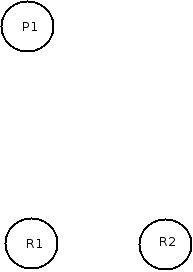
\includegraphics[scale=0.5]{images/acte1}
\end{itemize}
\subsection{Acte 2}
\begin{itemize}
  \bitem ordre = demande de ressources R1 par le processus P1 (O3)
  \bitem graphe = P1, R1, R2
  \bitem file R1 = P1
  \bitem règles = R3, R6, MV4 
  \bitem 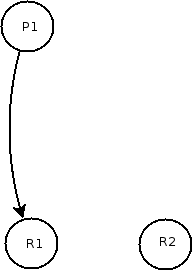
\includegraphics[scale=0.5]{images/acte2}
\end{itemize}
\subsection{Acte 3}
\begin{itemize}
  \bitem ordre = création d'un processus P2 (O1)
  \bitem graphe = P1, P2, R1, R2
  \bitem file R1 = P1
  \bitem règles = R2, MV1
  \bitem 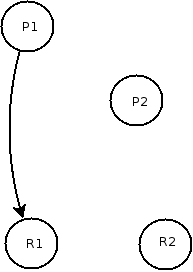
\includegraphics[scale=0.5]{images/acte3}
\end{itemize}
\subsection{Acte 4}
\begin{itemize}
  \bitem ordre = demande de ressources R1 et R2 par le processus P2
  \bitem graphe = P1, P2, R1, R2
  \bitem file R1 = P1, P2
  \bitem file R2 = P2
  \bitem règles = R1, R3, R4, R7, R8, MV5
  \bitem 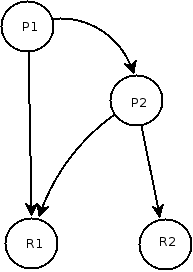
\includegraphics[scale=0.5]{images/acte4}
\end{itemize}
\subsection{Acte 5}
\begin{itemize}
  \bitem ordre = création d'un processus P3
  \bitem graphe = P1, P2, P3, R1, R2
  \bitem file R1 = P1, P2
  \bitem file R2 = P2
  \bitem règles = R2, R7, MV1
  \bitem 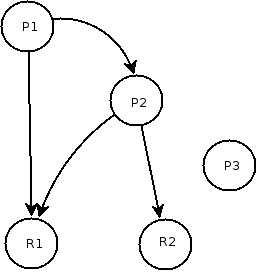
\includegraphics[scale=0.5]{images/acte5}
\end{itemize}
\subsection{Acte 6}
\begin{itemize}
  \bitem ordre = demande de ressources R2 par le processus P3
  \bitem graphe = P1, P2, P3, R1, R2
  \bitem file R1 = P1, P2
  \bitem file R2 = P2, P3
  \bitem règles = R1, R4, R7, MV5
  \bitem 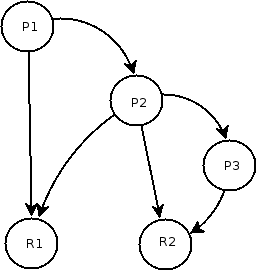
\includegraphics[scale=0.5]{images/acte6}
\end{itemize}
\subsection{Acte 7}
\begin{itemize}
  \bitem ordre = affichage des fils d'attente par ressources
  \bitem graphe = P1, P2, P3, R1, R2
  \bitem file R1 = P1, P2
  \bitem file R2 = P2, P3, P1
  \bitem règles = R7, MI9
\end{itemize}
\subsection{Acte 8}
\begin{itemize}
  \bitem ordre = demande de ressources R2 par le processus P1
  \bitem graphe = P1, P2, P3, R1, R2
  \bitem file R1 = P1, P2
  \bitem file R2 = P2, P3, P1
  \bitem règles = R1, R4, R7, R13, MV5
  \bitem 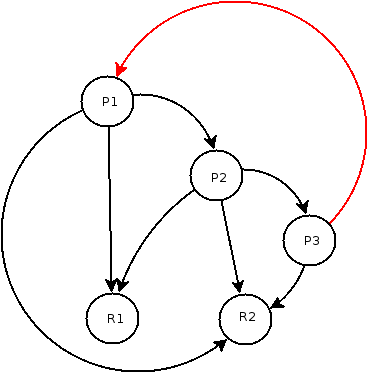
\includegraphics[scale=0.5]{images/acte8}
\end{itemize}
\subsection{Acte 9}
\begin{itemize}
  \bitem ordre = affichage des processsus concernés par un interblocage
  \bitem graphe = P1, P2, P3, R1, R2
  \bitem file R1 = P1, P2
  \bitem file R2 = P2, P3, P1
  \bitem règles = R7, MI8
\end{itemize}
\subsection{Acte 10}
\begin{itemize}
  \bitem ordre = destruction du processus P1
  \bitem graphe = P2, P3, R1, R2
  \bitem file R1 = P2
  \bitem file R2 = P2, P3
  \bitem règles = R7, R11, R12, MV2, MV3
  \bitem 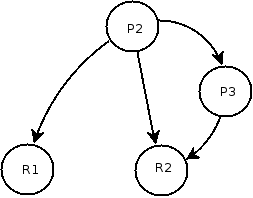
\includegraphics[scale=0.5]{images/acte10}
\end{itemize}
\subsection{Acte 11}
\begin{itemize}
  \bitem ordre = libération de la ressource R2 par le processsus P2
  \bitem graphe = P2, P3, R1, R2
  \bitem file R1 = P2
  \bitem file R2 = P3
  \bitem règles = R5, R7, R9, MV5, MV6
  \bitem 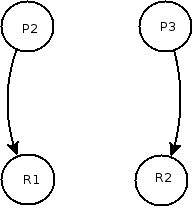
\includegraphics[scale=0.5]{images/acte11}
\end{itemize}
\subsection{Acte 12}
\begin{itemize}
  \bitem ordre = affichage des processsus actifs
  \bitem graphe = P2, P3, R1, R2
  \bitem file R1 = P2
  \bitem file R2 = P3
  \bitem règles = R6, MI3
\end{itemize}
\end{document}

